\documentclass[letterpaper]{article}

\usepackage{amsmath, amssymb}
\usepackage{nicefrac}
\usepackage{graphicx}
\usepackage{color}
\usepackage{listings}
\usepackage{float} %to stop image from moving
\usepackage{grffile}
\usepackage{enumitem}
\usepackage{cancel}
\usepackage{mathtools}
\usepackage{tikz}
\usepackage[a4paper]{geometry}

\PassOptionsToPackage{hyphens}{url}\usepackage{hyperref} %url is a sub-package

\begin{document}

\newgeometry{top=2cm,bottom=2cm}

\title{MATH 441: Project three (PDF/CDF)}
\author{James Starkman, jas497}
\date{2015-11-16}
\maketitle

%%%%%%%%%%%%%%%%%%%%%%%%%%%%%%%%%%%%%%%%%%%%%%%%%%%%%%%%%%%%%%%%%%%%%%%%%%%%%%%%
\section{Plots}
\label{sec:plots}

The structure of each figure is as follows.  The upper plot is the PDF, while
the lower is the CDF.  In both plots, the empirical distribution with a myriad
iterations is a histogram, while the rest are colored dots: red for ten
iterations, green for a hundred, and blue for a thousand.  The blue curve is the
mathematically-correct function (as best as the plotter and analytical
generating functions can draw it, anyways).  Magenta dots are for anything else.
This color scheme is consistent across all plots, and is defined in the
uppermost section of the code (included).

This section involves figures \ref{fig:dBinom}, \ref{fig:dPoiss},
\ref{fig:dDiceM}, \ref{fig:dNormG}, \ref{fig:dParet}, and \ref{fig:dGamma}.
Forty bins were always used unless stated otherwise.  Regarding discretization,
101 points were always used (100 intervals or ``slices''), except in the
comparison in the next section.

\begin{figure}[ht]
  \centering
  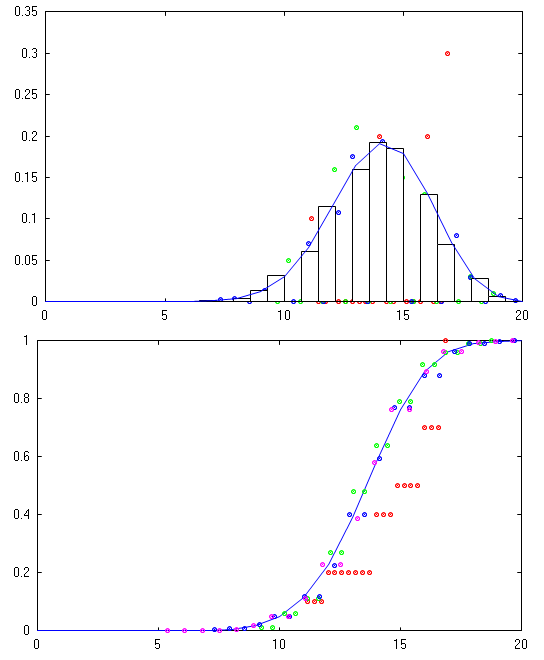
\includegraphics[width=\columnwidth]{2015-11-11_binomial.png}
  \caption{\label{fig:dBinom} Binomial distribution with $p=0.7, n=20$.
    Twenty-one buckets.  This particular distribution could probably use more
    simulations.}
\end{figure}

\begin{figure}[ht]
  \centering
  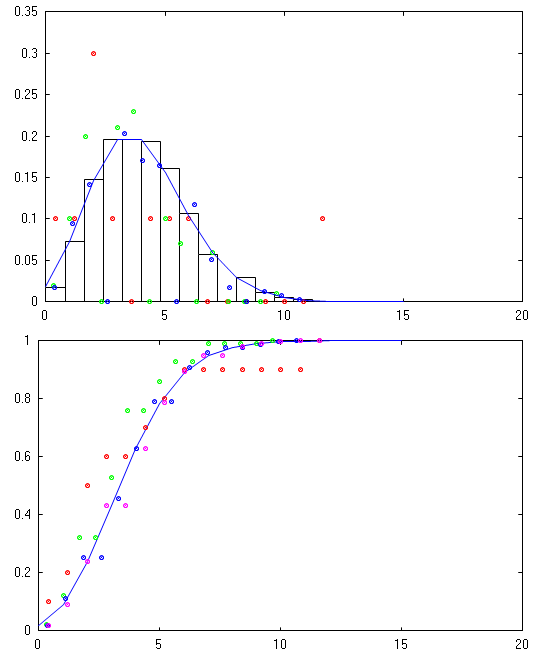
\includegraphics[width=\columnwidth]{2015-11-11_poisson.png}
  \caption{\label{fig:dPoiss} Poisson distribution with $\lambda=4$.  Fifteen
    bins because that looked reasonable when plotting.  The line appears
    segmented because only integer values on the x-axis were plotted (the rest
    were linearly-interpolated).}
\end{figure}

\begin{figure}[ht]
  \centering
  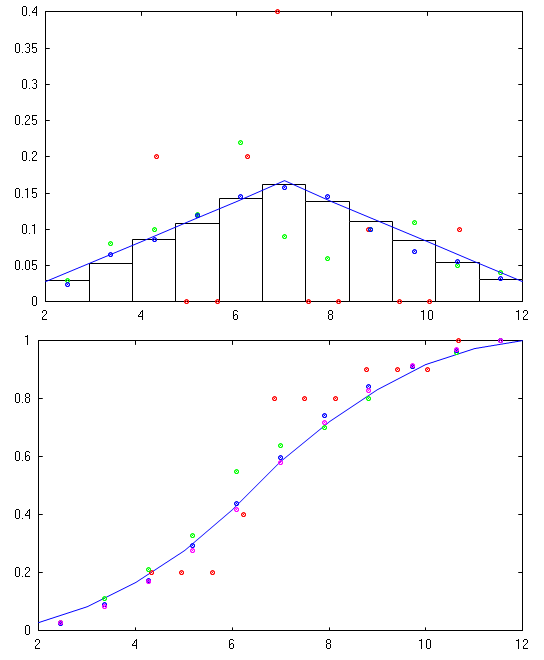
\includegraphics[width=\columnwidth]{2015-11-11_dice.png}
  \caption{\label{fig:dDiceM} Distribution of sum of two fair, six-sided dice.
    Eleven bins (since there are only eleven possible outcomes, 2--12
    inclusive).}
\end{figure}

\begin{figure}[ht]
  \centering
  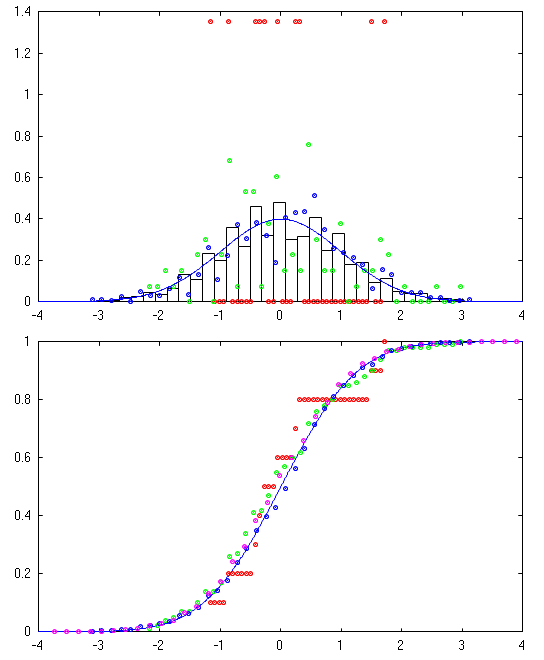
\includegraphics[width=\columnwidth]{2015-11-11_normal.png}
  \caption{\label{fig:dNormG} Normal distribution with $\mu=0, \sigma=1$.  This
    \emph{really} needs more than ten iterations, and to a greater extent than
    the other distributions; their red dots do not seem this \ldots\ off the
    mark in the others.  This is actually one of the better runs --- sometimes
    the red dots in the PDF went as high as three or four on the y-axis.}
\end{figure}

\begin{figure}[ht]
  \centering
  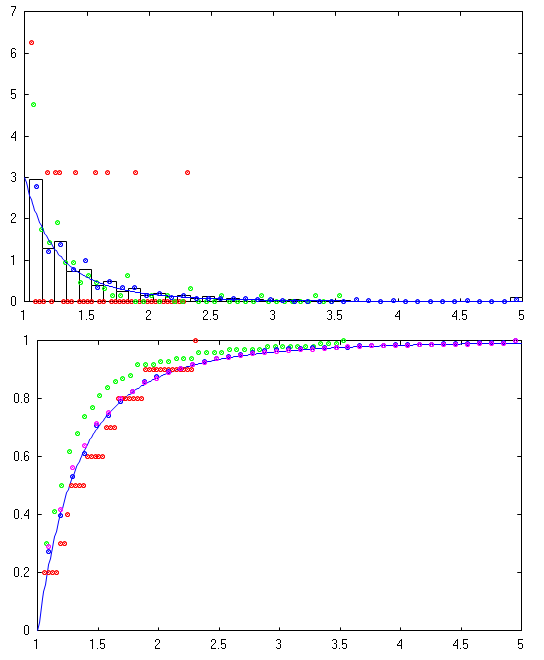
\includegraphics[width=\columnwidth]{2015-11-11_pareto.png}
  \caption{\label{fig:dParet} Pareto distribution with $\alpha=3$ and minimum
    value of one.}
\end{figure}

\begin{figure}[ht]
  \centering
  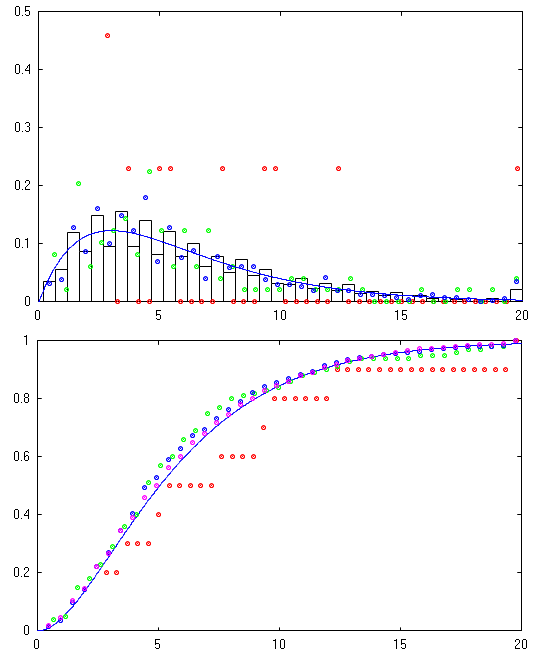
\includegraphics[width=\columnwidth]{2015-11-11_gamma.png}
  \caption{\label{fig:dGamma} Gamma distribution with $k=2, \theta=3$.}
\end{figure}
 
%%%%%%%%%%%%%%%%%%%%%%%%%%%%%%%%%%%%%%%%%%%%%%%%%%%%%%%%%%%%%%%%%%%%%%%%%%%%%%%%
\section{Exploration}
\label{sec:expl}

\subsection{Discretization}
\label{subsec:discrete}

This was done with the Normal distribution, for familiarity.

\begin{description}
\item[Two hundred slices] (More, closer together) Better than one hundred
  slices, but not by much.  Histogram heights are nearer the blue curve.
\item[One hundred slices] (Situation normal) See above figures.  Not too bad.
\item[Thirty slices] (Fewer, further apart) Not that bad, surprisingly.  The
  red/ten dots were even more erratic than usual, but the histogram/myriad
  followed the curve rather well.
\item[Ten slices] (Even fewer, even further apart) This barely looked Normal.
  Most bars in the histogram had a height of zero, although what few remained
  visible did loosely follow the Normal distribution.
\end{description}

\subsection{Other about samplers}
\label{subsec:othersamplers}

While they are clearly not perfect, the inverse CDF method works well enough.
Certainly, other methods (\emph{i.e.}, what Octave uses internally) converge
faster, but with enough brute force the Law of Large Numbers will eventually
give convergence.

The binomial sampler appears to need more than 10\,000 samples to become as
accurate as the others, while the dice rolling distribution was the closest to
reality.

The red/ten-iteration results were, generally, \emph{really bad}.  One should
never use that few if possible, as the Law of Large Numbers has not really
``kicked in'' yet.

\subsection{Compare with randn}
\label{subsec:randn}

See figure \ref{fig:cmpNorm}.  Octave uses a different algorithm, so the results
are expected to have different kinds of errors.  Visually, Octave's myriad of
numbers better approximate the Normal distribution than the inverse CDF's
myriad, and although the inverse method seemed to take longer to calculate, it
is still accurate.  That the built-in algorithm performs better is observation
bias; the programmers selected the best one they could find, and did not select
the rest.  Since parameter choices only apply linear transforms to the data
($\mu+z\sigma$), choice of parameters should not change the error appreciably.

\begin{figure}[ht]
  \centering
  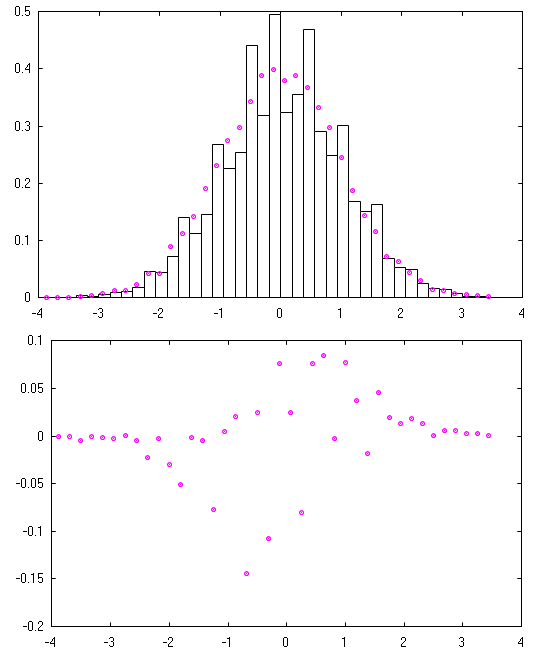
\includegraphics[width=\columnwidth]{2015-11-11_compare_normal.png}
  \caption{\label{fig:cmpNorm} Octave uses the Ziggurat algorithm, which appears
    to perform better than the ``normcdf()'' one used here.  Above: ``randn(1)''
    in magenta, superimposed on the empirical inverse CDF.  Below: difference
    (error) between ``randn'' and empirical distributions.}
\end{figure}

\restoregeometry

\clearpage

\newgeometry{left=1.5cm,top=2cm,bottom=2cm}

\section{Code}
\label{sec:code}

\lstinputlisting[language=Octave]{2015-11-11_tool.m}

\restoregeometry

\end{document}
